\documentclass[12pt, a4paper]{report}
\usepackage[utf8]{inputenc} % For Unicode characters
\usepackage{graphicx}       % For including images
\usepackage{hyperref}       % For clickable links in the PDF
\usepackage{amsmath}        % For mathematical symbols
\usepackage{caption}        % For custom captions
\usepackage{geometry}       % For page margins
\usepackage{float}
\usepackage{subfigure}
\usepackage{hyperref}
\geometry{a4paper, top = 1in, bottom = 1in, left = 1in, right = 1in}
\usepackage{hyperref}
\usepackage{ulem,graphicx}
\usepackage{}
\usepackage{xcolor}
\usepackage{titlesec}
\usepackage{microtype} % Prevents overfull hboxes by better text wrapping
\usepackage{subcaption}
\usepackage{color}
\usepackage{cite}
\usepackage{amsmath,amssymb,amsfonts}
\usepackage{algorithmic}
\usepackage{textcomp}
\usepackage{xcolor}
\usepackage{placeins}
\usepackage{graphicx}
\usepackage{subcaption}
\begin{document}



	
	% Title Page
	\begin{titlepage}
		\centering
		\vspace*{1.5in}
		{\Huge \textbf{JPEG IMAGE COMPRESSION}} \\[1cm]
		{\Large CS663 : Digital Image Processing} \\[1cm]
		\textbf{Prepared by:} \\[0.25cm]
		Toshan Achintya Golla(22B2234), Anupam Rawat(22B3982),\\ Amitesh Shekhar(22B0014) \\[0.5cm]
		\textbf{Date of Submission}\\[0.25cm]
		24 November 2024 \\[1.5cm]
		\vfill
	\end{titlepage}
	
	

	% Table of Contents
	\tableofcontents
	\newpage
	\chapter{Introduction}
	% Sections
	\section{Background}
	Image Compression has always been an important part of Digital Image Processing. Without compression, it is logistically impossible to store and transfer modern day media containers like images and videos. The size of raw videos and images, taken directly from the source, contains lot of redundant data which can be discarded without the loss of any meaningful information. For this project, we have worked on one of the most ubiquitous image compression standards, JPEG(Joint Photographic Experts Group). JPEG can easily achieve BPP (bits per pixel) of 1-2 for colored images without significant reduction in quality. Most webpages use jpeg standard for rendering images efficiently.
	\section{Problem Statement}
	 To build an image compression engine like JPEG and implement it for both grayscale and color images. \\ Analyse the quality of the compression using RMSE (Root Mean Squared Error) and BPP (Bits Per Pixel) plot.
	 
	\section{Structure of the Report}
	Our main goal is to implement a simple version of the JPEG algorithm, as was taught in the course. We start with first explaining the main blocks in the JPEG encoder and decoders in section 2.1 and a description of the algorithms used in section 2.2. The code description is given in section 3.1. The results are given in sections 4.1 (dataset used) and 4.2 (resulting images, performance curves etc.). The conclusion and comments are given in section 5.
	
	
	\chapter{Methodology}
	\section{Approach}
	Any general image compression model consists of two distinct functional components: an encoder and a decoder. The encoder performs the compression while the decoder performs the complementary operation of decompression. A block diagram is given below:
	\begin{figure}[H]
		\centering
		\includegraphics[width=0.7\linewidth]{jpeg_arch}
		\caption[functional block diagram of image compression model (ref: Gozalez and Woods)]{}
		\label{fig:jpegarch}
	\end{figure}
	
	In JPEG encoder, we use DCT (Discrete Cosine Transfom) to map the pixel data to its corresponding DCT coefficients. Then a quantizer block quantizes the coefficients (information is lost here, hence JPEG is a lossy compression algorithm). Finally, the quantized coefficients are encoded using run-length and Huffman coding scheme. This data is stored in a suitable format (.bin in our case). \\
	For the decoder block, the same steps are perfomed in the reverse order. (We have followed the scheme followed in class lectures).\newpage
	A block diagram of JPEG compression model is given below:
	\begin{figure}[H]
		\centering
		\includegraphics[width=1\linewidth]{jpeg_block_diagram.png}
		\caption{JPEG Compression Model (ref : Broko Furht, Research Gate)}
	\end{figure}
	
	\section{Algorithms Implemented}
	\begin{enumerate}
		\item \textbf{DCT-2D and IDCT-2D}\\
			We used the dct-2d() and idct-2d() functions from scipy library to implement discrete cosine transforms on the 8x8 patches. Internally, they use ffts to reduce time complexity.
		\item \textbf{Huffman Encoding}\\
			The quantized DCT coefficients were first arranged using \textbf{zig-zag} ordering. Now for each 8x8 patch, the Huffman encoding is done using a min-heap implementation.Again, as mentioned in the slides, separate encoding is done for DC and AC coefficients.
		\item \textbf{Reverse Huffman}\\
			The encoded coefficients are decoded by traversing the binary tree in reverse direction. The exact implementation is mentioned later.
	\end{enumerate}
	
	\chapter{Implementation}
	\section{JPEG Encoder}
	
	\begin{enumerate}
	\item Divide the image into 8x8 patches
		\begin{figure}[H]
			\centering
			\includegraphics[width=0.9\linewidth]{divide_into_blocks}
			\caption{}
			\label{fig:divideintoblocks}
		\end{figure}
	\item Use inbuilt functions of scipy to calculate dct coeffs of each block
	\item Quantize using the Quantization matrix and given Q-value
	\item Extract AC-components from each block, store in a list
	\item Extract all DC-components from each block, store in a list
	\item Perform Huffman encoding on AC-coefficients and get the ac-huffman-table:
	\begin{figure}[H]
		\centering
		\includegraphics[width=0.9\linewidth]{huffman_encoding_ac}
		\caption[ac_coeff huffman encoding]{}
		\label{fig:huffmanencodingac}
	\end{figure}
	\item Similarly perform huffman encoding for DC-coefficients (first item is untouched, rest are encoded using consecutive differences) .Finally get the dc-huffman-table
	
	\item Use run-length encoding to encode the coeffs into triplets and get ac and dc encoded values. Code for AC part given below:
\begin{figure}[H]
	\centering
	\includegraphics[width=0.9\linewidth]{run_length_ac}
	\caption[run length encoding for ac coefficients]{}
	\label{fig:runlengthac}
\end{figure}
	\item Create a header (in the form of dictionary) and store the final encoded blocks, dc-huffman-table, ac-huffman-table, Quality Factor and image shape in a .bin file.\begin{figure}[H]
		\centering
		\includegraphics[width=1\linewidth]{save_compressed_image}
		\caption[save the compressed file]{}
		\label{fig:savecompressedimage}
	\end{figure}
	
\end{enumerate}
	
	\section{JPEG Decoder}
	The same steps are perfomed, albeit in a reversed order. The main steps and important code snippets are given below:
	\begin{enumerate}
		\item Read the compressed bin file
		\item Extract the parameters of the image like image shape, quality factor, ac and dc huffman tables as well as the main encoded coefficients from the bin file.
		\begin{figure}[H]
			\centering
			\includegraphics[width=0.9\linewidth]{read_compressed_file}
			\caption[read compressed file]{}
			\label{fig:readcompressedfile}
		\end{figure}
		
		\item Decode the AC and DC coefficients using ac and dc huffman table and run-length decoding (as mentioned in Gonzalez and Woods)
		\begin{figure}[H]
			\centering
			\includegraphics[width=	1\linewidth]{decode_ac_coeffs}
			\caption[decode ac coefficients]{}
			\label{fig:decodeaccoeffs}
		\end{figure}
		\begin{figure}[H]
			\centering
			\includegraphics[width=1\linewidth]{decode_dc_coeffs}
			\caption[decode dc coefficients]{}
			\label{fig:decodedccoeffs}
		\end{figure}
		\item Decode each block using the previously obtained coefficients and reverse zig-zag
		\item Dequantize the coefficients (still error would be there due to rounding off during encoding)
		\item Inverse DCT
		\item Stitch the patches together to create the final decompressed image
		\begin{figure}[H]
			\centering
			\includegraphics[width=1\linewidth]{"stitch images"}
			\caption[stitch images]{}
			\label{fig:stitch-images}
		\end{figure}
	\end{enumerate}
	
	\section{JPEG for colored images}
	This \textbf{color JPEG compression} implementation is almost similar, with the following key differences from grayscale JPEG compression:
	
	\begin{enumerate}
		\item \textbf{Color Space Conversion}: 
		The input color image (in BGR format) is converted to the \textbf{YCbCr color space}, separating luminance (Y) and chrominance (Cb, Cr) components (using an inbuilt function of opencv $.COLOR_BGR2YCrCb$) which internally uses similar formula as the one mentioned in the slides :
		\begin{align*}
			Y &= 16 + (65.481R + 128.553G + 24.966B) \\
			C_B &= 128 + (-37.79R - 74.203G + 112B) \\
			C_R &= 128 + (112R - 93.786G - 18.214B)
		\end{align*}
		
		\item \textbf{Chroma Subsampling}: 
		The chrominance channels (Cb and Cr) are \textbf{downsampled} (halved) to reduce data size while retaining visual quality. This step is not required for grayscale images.
		
		\item \textbf{Separate Compression}: 
		Each channel (Y, downsampled Cb, and downsampled Cr) undergoes compression using a \textbf{grayscale JPEG compression} method independently.
		
		\item \textbf{Upsampling}: 
		The chrominance channels are \textbf{upsampled} back to their original dimensions after processing to reconstruct the image.
		
		\item \textbf{Final Reconstruction}: 
		The compressed YCbCr image is merged and converted back to the BGR format for saving as the final compressed image.
	\end{enumerate}
	
	By handling chrominance data separately and using subsampling, color JPEG achieves greater \textbf{compression efficiency} compared to grayscale JPEG, while maintaining visual fidelity.
	
	
	\chapter{Results and Analysis}
	
	\section{JPEG on grayscale images}
	Original Image: (note that we have first converted it to grayscale using \href{https://blackandwhite.imageonline.co/}{this} and then used it for our jpeg compressor since the inbuilt function of opencv for grayscale conversion was introducting some white dots in the compressed images.)
	\begin{figure}[H]
		\centering
		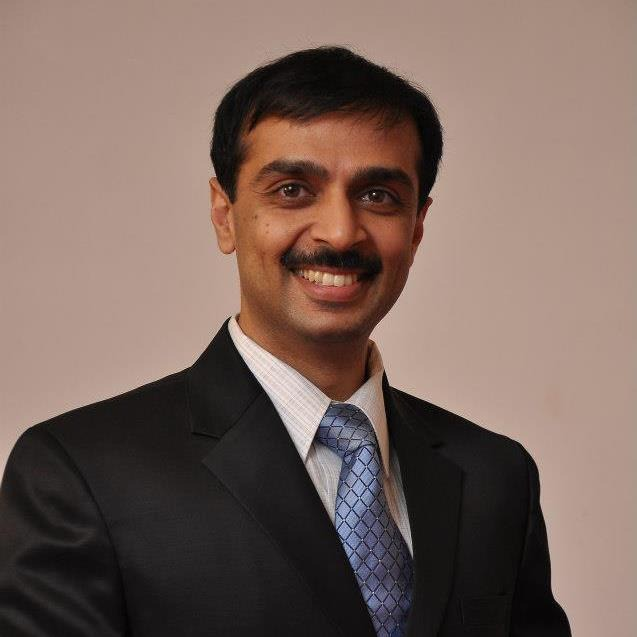
\includegraphics[width=0.5\linewidth]{ajit}
		\caption{Original Image, Size = 42KB, 637x637 image (credits : Professor Ajit Rajwade, IIT Bombay)}
	\end{figure}
	\newpage
	JPEG Compression for increasing Q (quality factor):
	\begin{figure}[H]
		\centering
		\setlength{\tabcolsep}{1pt} % Adjust spacing between images
		\renewcommand{\arraystretch}{0} % Remove vertical spacing
		\begin{tabular}{ccc}
			\subfigure[Q = 10, 19KB]{\includegraphics[width=0.3\textwidth]{Compressed_image_10.jpg}} &
			\subfigure[Q = 20, 22KB]{\includegraphics[width=0.3\textwidth]{Compressed_image_20.jpg}} &
			\subfigure[Q = 30, 26KB]{\includegraphics[width=0.3\textwidth]{Compressed_image_30.jpg}} \\
			\subfigure[Q = 40, 29KB]{\includegraphics[width=0.3\textwidth]{Compressed_image_40.jpg}} &
			\subfigure[Q = 50, 32KB]{\includegraphics[width=0.3\textwidth]{Compressed_image_50.jpg}} &
			\subfigure[Q = 60, 36KB]{\includegraphics[width=0.3\textwidth]{Compressed_image_60.jpg}} \\
			\subfigure[Q = 70, 37KB]{\includegraphics[width=0.3\textwidth]{Compressed_image_70.jpg}} &
			\subfigure[Q = 80, 40KB]{\includegraphics[width=0.3\textwidth]{Compressed_image_80.jpg}} &
			\subfigure[Q = 90, 41KB]{\includegraphics[width=0.3\textwidth]{Compressed_image_90.jpg}} \\
			\subfigure[Q = 100, 41KB]{\includegraphics[width=0.3\textwidth]{Compressed_image_100.jpg}}&
			\subfigure[Q = 300, 51KB]{\includegraphics[width=0.3\textwidth]{Compressed_image_300.jpg}}&
			\subfigure[Q = 500, 51KB]{\includegraphics[width=0.3\textwidth]{Compressed_image_500.jpg}}\\
		\end{tabular}
		\caption{Compressed Images for increasing Q (10 to 100 in steps of 10 from top to bottom, left to right)}
		\label{fig:5x2_grid}
	\end{figure}
	\subsection{Dataset Used for the RMSE vs BPP plot}
	We have used the \href{https://r0k.us/graphics/kodak/}{Kodak Lossless True Color Image Suite} dataset. They are lossless, true color (24 bits per pixel, aka "full color") images in png format (since it a lossless standard). Each image is 768x512 or 512x768 in size and we have used 24 images from this suite.
	\subsection{RMSE vs BPP plot}
	\begin{figure}[H]
		\centering
		\includegraphics[width=1\textwidth]{grayscale_rmse_vs_bpp}
		\caption{RMSE vs BPP plot for Grayscale images from the kodak dataset}
	\end{figure}
	\newpage
		\section{JPEG on color images}
	Original Image: 
	\begin{figure}[H]
		\centering
		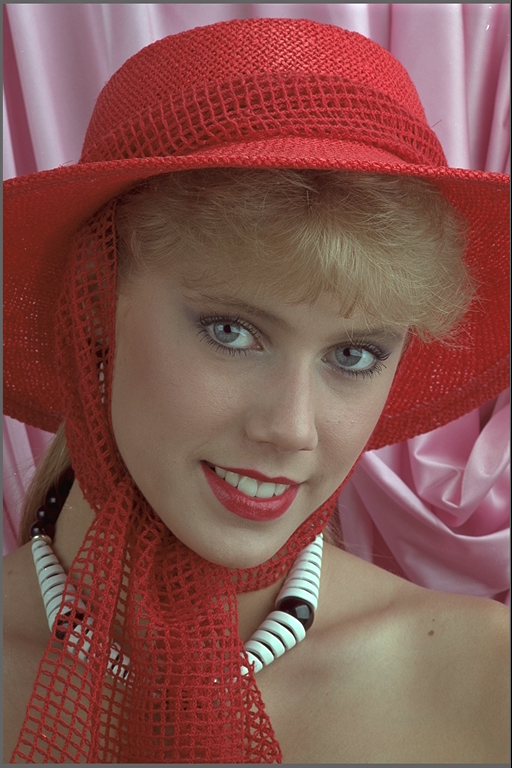
\includegraphics[width=0.5\linewidth]{kodim04}
		\caption{Original Image, Size = 623KB, 512x768 image}
	\end{figure}
	\newpage
	JPEG Compression for increasing Q (quality factor):
	\begin{figure}[H]
		\centering
		\setlength{\tabcolsep}{5pt} % Adjust spacing between images
		%\renewcommand{\arraystretch}{3pt} % Remove vertical spacing
		\begin{tabular}{ccc}
			\subfigure[Q = 10, 38KB]{\includegraphics[width=0.3\textwidth]{Color_Compressed_image_10.jpg}} &
			\subfigure[Q = 30, 72KB]{\includegraphics[width=0.3\textwidth]{Color_Compressed_image_30.jpg}} &
			\subfigure[Q = 50, 90KB]{\includegraphics[width=0.3\textwidth]{Color_Compressed_image_50.jpg}} \\
			\subfigure[Q = 70, 102KB]{\includegraphics[width=0.3\textwidth]{Color_Compressed_image_70.jpg}} &
			\subfigure[Q = 90, 109KB]{\includegraphics[width=0.3\textwidth]{Color_Compressed_image_90.jpg}} &
			\subfigure[Q = 110, 118KB]{\includegraphics[width=0.3\textwidth]{Color_Compressed_image_110.jpg}} \\
		\end{tabular}
		\caption{Compressed Images for increasing Q (10 to 110 in steps of 20 from top to bottom, left to right)}
		\label{fig:5x2_grid}
	\end{figure}
	\subsection{Dataset Used for the RMSE vs BPP plot}
	We have used the same \href{https://r0k.us/graphics/kodak/}{Kodak Lossless True Color Image Suite} dataset. They are lossless, true color (24 bits per pixel, aka "full color") images in png format (since it a lossless standard). Each image is 768x512 or 512x768 in size and we have used 24 images from this suite.
	\subsection{RMSE vs BPP plot}
	\begin{figure}[H]
		\centering
		\includegraphics[width=1\textwidth]{color_rmse_vs_bpp}
		\caption{RMSE vs BPP plot for Color images from the kodak dataset}
	\end{figure}
	
	
	\chapter{Conclusion}
	We successfully implemented the JPEG algorithm, achieving 0.65 BPP for grayscale image at Q=50 and 1.8 BPP for color image at Q=50. This is a tremendous level of compression without much loss in information.
	Some of the good and bad aspects of our implementation are as follows:\\
	\textbf{Good Aspects}
	\begin{enumerate}
		\item Implementation in python as opposed to cpp or matlab. Makes the code easier to follow and understand. Matrix manipulation is taken care by numpy. Also faster due to parallel computation (not relevant for our tiny workload though).
		\item Using heaps to implement Huffman encoding. Since heaps also store the data as a min-max binary tree, it is exactly similar to the huffman tree. Implemeting heap is also made easier by python's inbuilt library and its compatibility with multi-dimensional lists.
		\item Code is modular, script can be directly imported as a module
		\item Made a interactive GUI using tkinter library, makes the demo more presentable and elegant.
		\item Ringing and seam artifacts are minimized at Q above 30 (according to our limited testing)
	\end{enumerate}
	\textbf{Bad Aspects}
	\begin{enumerate}
		\item We are cropping the image to make the height and width multiples of 8. This leads to loss of information (though unavoidable in our model). Padding could have been a better approach.
		\item Upon converting RGB to grayscale images using the inbuilt function of opencv (or averaging the R,G, B values) was leading to small scattered dots in the output image (But doing so using online converter tools avoided this issue). There may exist a better way to convert from RGB colorspace to grayscale which prevents this.
		\item Implementing the code in good old C would have lead to a more efficient and faster code.
	\end{enumerate}
	\chapter{Contributions}
	\begin{enumerate}
		\item Toshan Achintya Golla (22b2234) : Wrote the code for encoder, saving the compressed file in bin format (earlier decided on JSON) and decoder, implemented color compression
		\item Anupam Rawat (22b3982) : Reconstruction and Combination of the image patches, Made the interactive GUI, result analysis
		\item Amitesh Shekhar (22b0014) : Huffman encoding-decoding and run-length encoding, Report, Read the research paper : \textit{Using partial differential equations (PDEs) for image compression: M. Mainberger and J.Weickert, "Edge-Based Image Compression with Homogeneous Diffusion", CAIP 2009}
	\end{enumerate}
	
\end{document}
